\documentclass[uplatex,9pt]{jsarticle}
\usepackage{resume}
\usepackage{udline}
\usepackage{comment}
\usepackage[margin=0pt,font=small]{caption}
\usepackage{titlesec}
\usepackage{graphicx}
\usepackage{indentfirst}


\pagestyle{plain}

\titlespacing*{\section}{0pt}{6pt}{4pt}
\titlespacing*{\subsection}{0pt}{4pt}{2pt}

\setlength\intextsep{4pt}
\setlength\textfloatsep{4pt}
\setlength\floatsep{4pt}
\setlength{\parindent}{1zw}



\begin{document}

\twocolumn[
    \beginheader{2026年度 コンピュータサイエンス学部 中中間発表}{2026}{6}{19}{井上 研究室}
    \title{VRにおける攻撃エフェクトの表示手法が視認性とゲーム体験に与える影響}
    \author{C0B23049 北村 晴貴 (Haruki Kitamura)}
    \endheader
]
\vspace{3mm}
\setcounter{page}{15}
\AtBeginDocument{\setlength{\parindent}{1zw}}


\section{はじめに}

近年，VRゲームの普及に伴い，高い没入感を活かしたゲーム体験が求められている．その中で，炎やビームなどの攻撃エフェクトは，戦闘の迫力や臨場感を高める演出として広く利用されており，大きく表現される場合がある．

しかし，大規模な攻撃エフェクトはプレイヤー自身の視界を遮る可能性がある．特に一人称視点では，攻撃中に対象物や周囲の状況が見えにくくなり，ターゲットの追従や照準操作が困難になることが考えられる．その結果，視認性や操作性の低下につながる可能性がある．

VRにおける視認性や情報提示に関する研究は数多く行われているが，ユーザ自身が生成する攻撃エフェクトによる視界遮蔽については十分に検討されていない．また，遮蔽を軽減するために攻撃エフェクトを透明化した場合，攻撃の迫力や没入感が損なわれる可能性がある．

そこで本研究では，自己生成攻撃エフェクトによる視界遮蔽に着目し，攻撃エフェクトの表示方法が視認性およびゲーム体験に与える影響を調査する．さらに，視認性とゲーム体験を両立できる攻撃エフェクトの表示手法について検討する．

\section{関連研究}

\begin{figure}[htbp]
\begin{center}
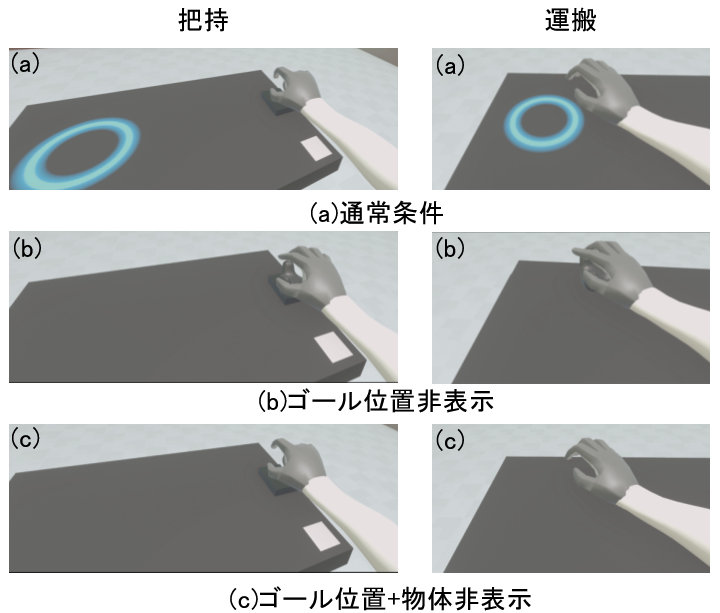
\includegraphics[width=0.85\linewidth]{fig/act5.png}
\caption{可視性についての各条件}
\label{fig:act5}
\end{center}
\end{figure}

VR空間では，ユーザが取得できる視覚情報が操作性能に影響することが知られている．湯村らは自己身体および目標位置の可視性に着目し，それらが可視な環境では物体操作精度が向上することを示した\cite{yumura2021visibility}．この結果は，ユーザが利用できる視覚情報量とタスク成績との関連を示唆している(\figref{fig:act5})．

\begin{figure}[htbp]
\begin{center}
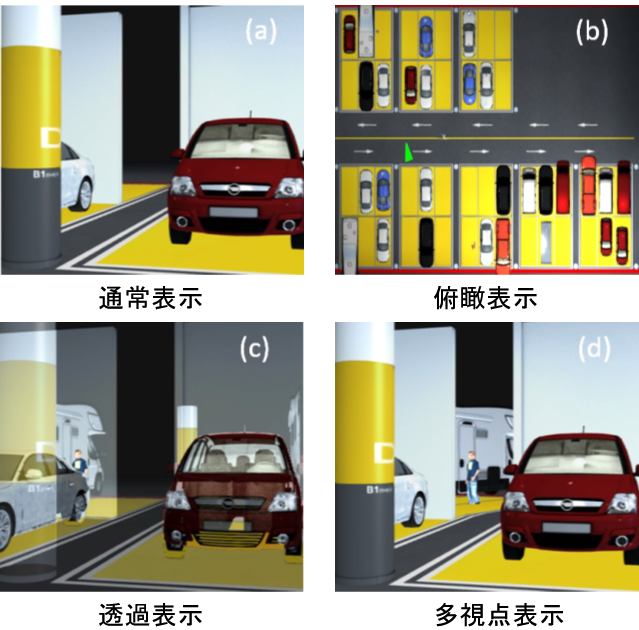
\includegraphics[width=0.85\linewidth]{fig/act6.png}
\caption{遮蔽可視化手法の比較}
\label{fig:act6}
\end{center}
\end{figure}

一方，遮蔽物によって対象が見えなくなる遮蔽問題が課題として扱われている．Wangらは，対象物を半透明表示や別視点表示によって可視化する手法を比較し，可視化方法によって探索効率や対象発見性能が変化することを報告している\cite{wang2019occlusion}．このように，遮蔽そのものだけでなく，遮蔽された対象をどのように提示するかも重要な検討事項である(\figref{fig:act6}).

しかし，既存研究では環境中の物体による遮蔽が主に扱われており，ユーザ自身が発生させる攻撃エフェクトによる遮蔽については十分に検討されていない．また，攻撃エフェクトは単なる遮蔽物ではなく，ゲームの迫力や没入感を構成する演出要素でもある．

そのため，視認性の向上だけでなく，ゲーム体験への影響も考慮した攻撃エフェクトの設計が求められる．そこで本研究では，攻撃エフェクトの表示方法に着目し，視認性とゲーム体験の両面から評価を行う．

\section{攻撃エフェクト表示手法}

\subsection{システム概要}
本研究では，攻撃エフェクトによる視界遮蔽が視認性およびゲーム体験に与える影響を調査する．プレイヤーは攻撃エフェクトを発生させながら移動するターゲットを追従し，各表示条件を比較する．

\subsection{攻撃エフェクトの表示条件}
攻撃エフェクトは対象物を遮蔽し，視認性を低下させる可能性がある．そこで本研究では，攻撃エフェクトの表示方法を変更し，視界遮蔽の影響を軽減することを試みる．

比較する表示条件は，通常表示，半透明表示，部分透過表示，輪郭表示の4種類である．
半透明表示では攻撃エフェクト全体の透過度を変更し，本研究では25\%，50\%，75\%の条件を用いる(\figref{fig:act7}).透過度が高いほどターゲットは見やすくなる一方で，攻撃の迫力が低下する可能性がある．
部分透過表示では，ターゲットと重なっている部分のエフェクトのみを透過表示する．
輪郭表示では，攻撃エフェクトによって隠れたターゲットの輪郭を強調表示する．
これらの表示条件を比較することで，視認性とゲーム体験を両立できる表示手法について検討する．

\begin{figure}[htbp]
\begin{center}
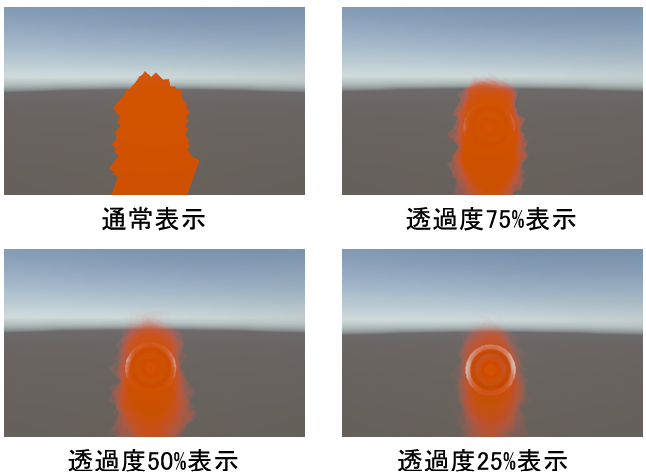
\includegraphics[width=0.85\linewidth]{fig/act7.png}
\caption{半透明表示の比較}
\label{fig:act7}
\end{center}
\end{figure}



\section{実装}

本研究では，Unityを用いてブレス攻撃環境を実装した．プレイヤーは攻撃エフェクトを発生させることができ，攻撃によってターゲットが遮蔽される状況を再現している．
また，評価実験で使用するターゲット追従タスクも実装した．ターゲットは一定範囲内を移動し，5秒ごとに移動方向を変更する．
現在はPC環境で実装を行っており，矢印キーによって攻撃方向を操作し，キーボード入力によって攻撃を発生させる．
さらに，通常表示および半透明表示の実装が完了しており，今後は部分透過表示および輪郭表示の実装を進める予定である．

\section{実験手順}

被験者には，各表示条件においてターゲット追従タスクを行ってもらう．
タスクでは，画面内を移動するターゲットに対して攻撃を行いながら，30秒間継続して追従する．ターゲットは一定範囲内を移動し，5秒ごとに移動方向をランダムに変更する．
被験者は攻撃エフェクトによる視界遮蔽の影響を受けながら，ターゲットを見失わないよう追従する．
各表示条件について同様のタスクを実施し，その後主観評価アンケートに回答してもらう．


\section{評価方法}

\subsection{客観評価}

視認性の評価にはターゲット追従誤差を用いる(\figref{fig:act8})．
追従誤差はターゲット中心と照準中心との距離として定義し，値が小さいほどターゲットを正確に視認し，追従できていることを示す．
各表示条件における追従誤差を比較することで，表示方法が視認性に与える影響を評価する．

\begin{figure}[htbp]
\begin{center}
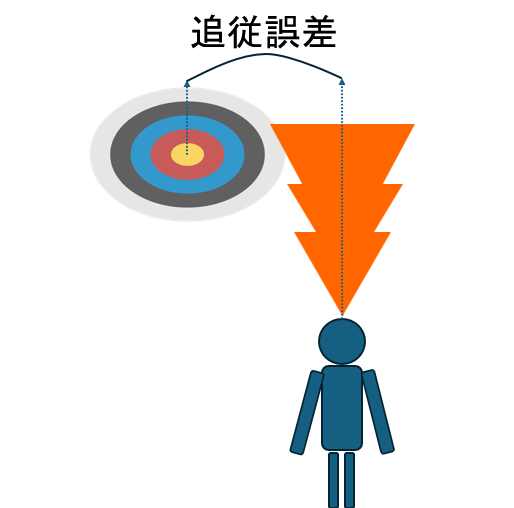
\includegraphics[width=0.68\linewidth]{fig/act8.png}
\caption{追従誤差の説明}
\label{fig:act8}
\end{center}
\end{figure}

\subsection{主観評価}

タスク終了後にアンケートを実施する．
評価項目は視認性，没入感，迫力，満足度の4項目とし，各項目について7段階評価で回答してもらう．
主観評価結果を比較することで，各表示条件がゲーム体験に与える影響を評価する．

\section{まとめ}

本研究では，攻撃エフェクトによる視界遮蔽に着目し，視認性とゲーム体験の両立を目的とした表示手法について検討した．
そのために，通常表示，半透明表示，部分透過表示，輪郭表示の複数の表示条件を用いたブレス攻撃環境を構築した．

今後は部分透過表示および輪郭表示の実装を進めるとともに，評価実験を実施し，各表示条件が視認性およびゲーム体験に与える影響について調査する予定である．

\bibliographystyle{junsrt}
\bibliography{ref}

\end{document}
